\section{Method}
\subsection{The experimental setup}

\begin{figure}
    \centering
    \begin{subfigure}[b]{0.4\textwidth}
        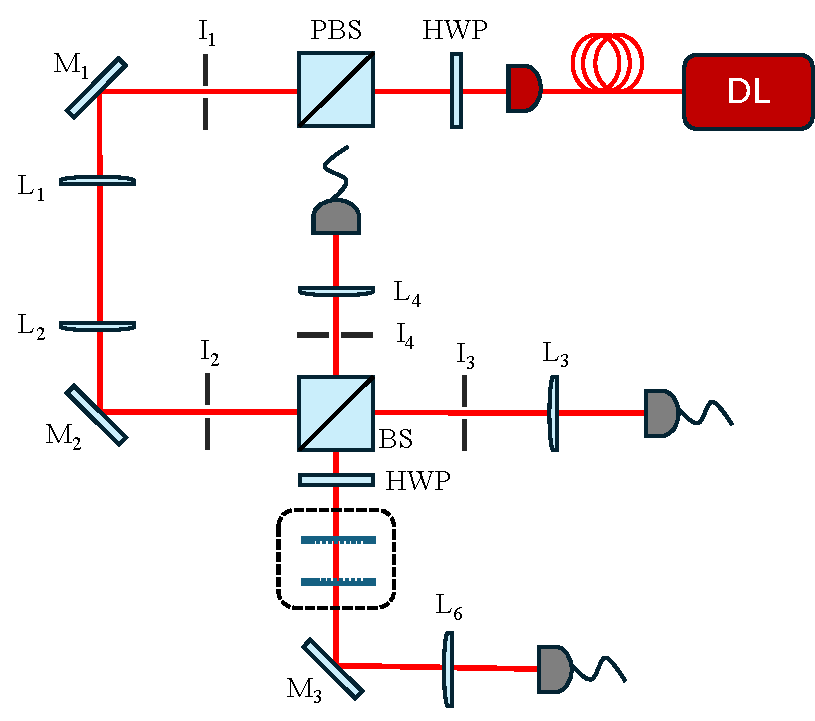
\includegraphics[width=\textwidth]{figures/setup_sketch.pdf}
        \caption{Schematics of the experimental setup for measuringthe transmission through a double fano cavity. The cavity setup shown in (b) is located in position marked by the dotted line.}
    \end{subfigure}
    \hfill
    \begin{subfigure}[b]{0.59\textwidth}
        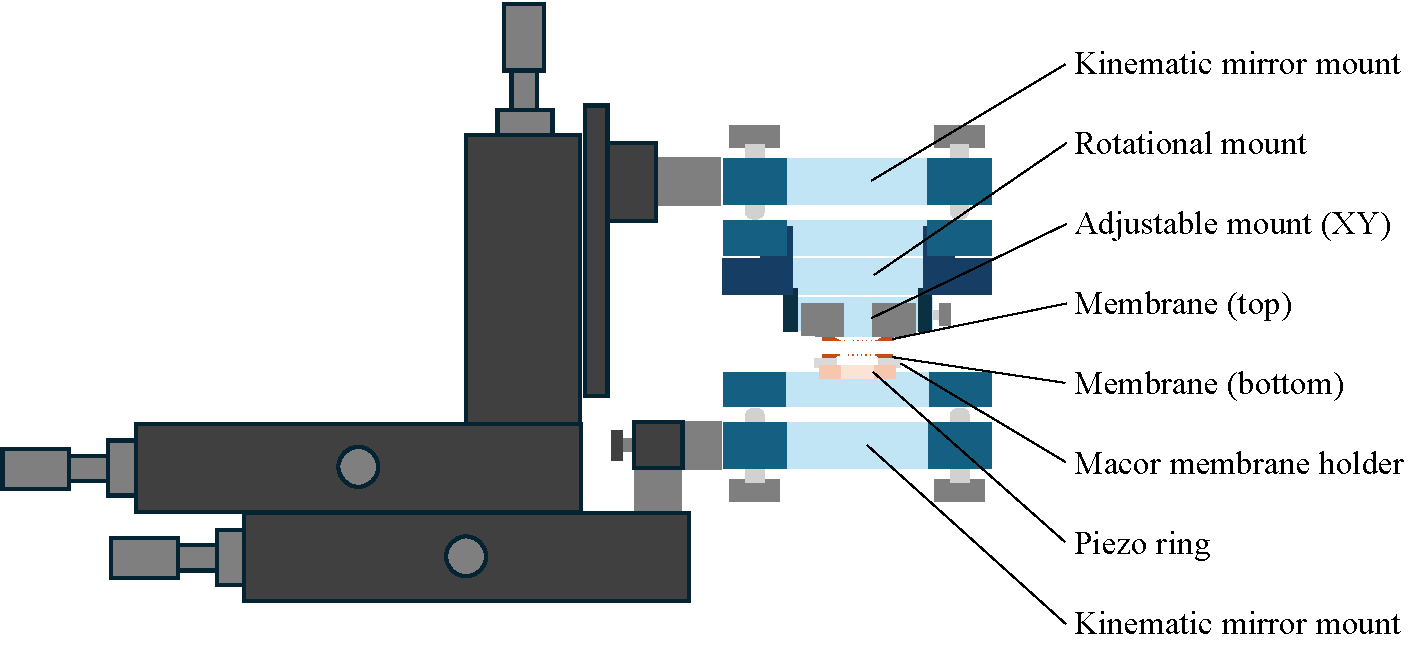
\includegraphics[width=\textwidth]{figures/setup_skecth_zoomed.pdf}
        \caption{Sketch of the part of the experimental setup containing the optical cavity.}
    \end{subfigure}
\end{figure}

\subsection{Characterization of sub-wavelength grating}

Figures:
\begin{itemize}
    \item Pictures of the membrane before patterning.
    \item AFM profile of the grating after patterning. (talk about profilometry and the physical parameters of the grating and their meaning for project).
    \item MAYBE: MIST simulation showing that the model accurately predicts the simulated spectra.
\end{itemize}

\subsubsection{Obtaining normalized transmission/reflection spectra}

\subsubsection{Adjusting the beam waist - the optical telescope}

\subsubsection{The alignment procedure}

\subsubsection{Normalization}

\subsection{Cavity measurements}

\subsubsection{Determining the cavity length from the FSR}

Figures: 
\begin{itemize}
    \item Linewidth as a function of "time" - to see the reduction of the linewidth as the piezo reaches an equilibrium where any time-dependent drift is reduced. 
\end{itemize}

\subsubsection{Normalization}

\subsubsection{Single fano cavity characterization} 

\subsubsection{Aligning the cavity}

Incluce: 
\begin{itemize}
    \item Scan for optimal cavity length
    \item Measure the spectral linewidth
    \item 
\end{itemize}

\subsubsection{Double fano cavity characterization}

\subsubsection{Off-resonance Fabry-Perot cavity (alignment technique)}

\subsubsection{Centering of the top grating (pinhole method)}

\subsection{Parallelism study (deviation from normal incident)}